\documentclass[twoside]{book}

% Packages required by doxygen
\usepackage{fixltx2e}
\usepackage{calc}
\usepackage{doxygen}
\usepackage[export]{adjustbox} % also loads graphicx
\usepackage{graphicx}
\usepackage[utf8]{inputenc}
\usepackage{makeidx}
\usepackage{multicol}
\usepackage{multirow}
\PassOptionsToPackage{warn}{textcomp}
\usepackage{textcomp}
\usepackage[nointegrals]{wasysym}
\usepackage[table]{xcolor}

% Font selection
\usepackage[T1]{fontenc}
\usepackage[scaled=.90]{helvet}
\usepackage{courier}
\usepackage{amssymb}
\usepackage{sectsty}
\renewcommand{\familydefault}{\sfdefault}
\allsectionsfont{%
  \fontseries{bc}\selectfont%
  \color{darkgray}%
}
\renewcommand{\DoxyLabelFont}{%
  \fontseries{bc}\selectfont%
  \color{darkgray}%
}
\newcommand{\+}{\discretionary{\mbox{\scriptsize$\hookleftarrow$}}{}{}}

% Page & text layout
\usepackage{geometry}
\geometry{%
  a4paper,%
  top=2.5cm,%
  bottom=2.5cm,%
  left=2.5cm,%
  right=2.5cm%
}
\tolerance=750
\hfuzz=15pt
\hbadness=750
\setlength{\emergencystretch}{15pt}
\setlength{\parindent}{0cm}
\setlength{\parskip}{3ex plus 2ex minus 2ex}
\makeatletter
\renewcommand{\paragraph}{%
  \@startsection{paragraph}{4}{0ex}{-1.0ex}{1.0ex}{%
    \normalfont\normalsize\bfseries\SS@parafont%
  }%
}
\renewcommand{\subparagraph}{%
  \@startsection{subparagraph}{5}{0ex}{-1.0ex}{1.0ex}{%
    \normalfont\normalsize\bfseries\SS@subparafont%
  }%
}
\makeatother

% Headers & footers
\usepackage{fancyhdr}
\pagestyle{fancyplain}
\fancyhead[LE]{\fancyplain{}{\bfseries\thepage}}
\fancyhead[CE]{\fancyplain{}{}}
\fancyhead[RE]{\fancyplain{}{\bfseries\leftmark}}
\fancyhead[LO]{\fancyplain{}{\bfseries\rightmark}}
\fancyhead[CO]{\fancyplain{}{}}
\fancyhead[RO]{\fancyplain{}{\bfseries\thepage}}
\fancyfoot[LE]{\fancyplain{}{}}
\fancyfoot[CE]{\fancyplain{}{}}
\fancyfoot[RE]{\fancyplain{}{\bfseries\scriptsize Generated by Doxygen }}
\fancyfoot[LO]{\fancyplain{}{\bfseries\scriptsize Generated by Doxygen }}
\fancyfoot[CO]{\fancyplain{}{}}
\fancyfoot[RO]{\fancyplain{}{}}
\renewcommand{\footrulewidth}{0.4pt}
\renewcommand{\chaptermark}[1]{%
  \markboth{#1}{}%
}
\renewcommand{\sectionmark}[1]{%
  \markright{\thesection\ #1}%
}

% Indices & bibliography
\usepackage{natbib}
\usepackage[titles]{tocloft}
\setcounter{tocdepth}{3}
\setcounter{secnumdepth}{5}
\makeindex

% Hyperlinks (required, but should be loaded last)
\usepackage{ifpdf}
\ifpdf
  \usepackage[pdftex,pagebackref=true]{hyperref}
\else
  \usepackage[ps2pdf,pagebackref=true]{hyperref}
\fi
\hypersetup{%
  colorlinks=true,%
  linkcolor=blue,%
  citecolor=blue,%
  unicode%
}

% Custom commands
\newcommand{\clearemptydoublepage}{%
  \newpage{\pagestyle{empty}\cleardoublepage}%
}

\usepackage{caption}
\captionsetup{labelsep=space,justification=centering,font={bf},singlelinecheck=off,skip=4pt,position=top}

%===== C O N T E N T S =====

\begin{document}

% Titlepage & ToC
\hypersetup{pageanchor=false,
             bookmarksnumbered=true,
             pdfencoding=unicode
            }
\pagenumbering{alph}
\begin{titlepage}
\vspace*{7cm}
\begin{center}%
{\Large Implementation of Dijsktra\textquotesingle{}s algorithm using Binary, Binomial and Fibonacci Heaps \\[1ex]\large Anant Maheshwari 13\+C\+O111 Shrukul Habib 13\+C\+O143 }\\
\vspace*{1cm}
{\large Generated by Doxygen 1.8.12}\\
\end{center}
\end{titlepage}
\clearemptydoublepage
\pagenumbering{roman}
\tableofcontents
\clearemptydoublepage
\pagenumbering{arabic}
\hypersetup{pageanchor=true}

%--- Begin generated contents ---
\chapter{Class Index}
\section{Class List}
Here are the classes, structs, unions and interfaces with brief descriptions\+:\begin{DoxyCompactList}
\item\contentsline{section}{\hyperlink{classBinomialHeap}{Binomial\+Heap} \\*Binomial Heap Data Structure class }{\pageref{classBinomialHeap}}{}
\item\contentsline{section}{\hyperlink{classFibonacciHeap}{Fibonacci\+Heap} \\*Fibonacci Heap Data Structure class }{\pageref{classFibonacciHeap}}{}
\item\contentsline{section}{\hyperlink{structnode}{node} \\*$\ast$-\/-\/-\/-\/-\/-\/-\/-\/-\/-\/-\/-\/-\/-\/-\/-\/-\/-\/-\/-\/-\/-\/-\/-\/-\/------B\+I\+N\+O\+M\+I\+AL H\+E\+A\+P-\/-\/-\/-\/-\/-\/-\/-\/-\/-\/-\/-\/-\/-\/-\/-\/-\/-\/-\/-\/-\/-\/-\/-\/-\/-\/-\/-\/-\/-\/-\/-\/-\/-\/-\/-\/-\/-\/-\/-\/-\/-\/-\/-\/-\/-\/-\/-\/-\/-\/------$\ast$/ }{\pageref{structnode}}{}
\item\contentsline{section}{\hyperlink{structnodef}{nodef} \\*$\ast$-\/-\/-\/-\/-\/-\/-\/-\/-\/-\/-\/-\/-\/-\/-\/-\/-\/-\/-\/-\/-\/-\/-\/-\/-\/-\/------F\+I\+B\+O\+N\+A\+C\+CI H\+E\+A\+P-\/-\/-\/-\/-\/-\/-\/-\/-\/-\/-\/-\/-\/-\/-\/-\/-\/-\/-\/-\/-\/-\/-\/-\/-\/-\/-\/-\/-\/-\/-\/-\/-\/-\/-\/-\/-\/-\/-\/-\/-\/-\/-\/-\/-\/-\/-\/-\/-\/-\/-\/-\/-\/-\/-\/-\/-\/-\/-\/-\/-\/-\/-\/------$\ast$/ }{\pageref{structnodef}}{}
\end{DoxyCompactList}

\chapter{File Index}
\section{File List}
Here is a list of all documented files with brief descriptions\+:\begin{DoxyCompactList}
\item\contentsline{section}{\hyperlink{red__black__tree_8c}{red\+\_\+black\+\_\+tree.\+c} \\*Implementation of Red Black Tree }{\pageref{red__black__tree_8c}}{}
\end{DoxyCompactList}

\chapter{Class Documentation}
\hypertarget{classBinomialHeap}{}\section{Binomial\+Heap Class Reference}
\label{classBinomialHeap}\index{Binomial\+Heap@{Binomial\+Heap}}


Binomial Heap Data Structure class.  


\subsection*{Public Member Functions}
\begin{DoxyCompactItemize}
\item 
\hyperlink{structnode}{node} $\ast$ \hyperlink{classBinomialHeap_a3ffaab6756189d14dd76e4e7a48147b6}{Initializeheap} ()
\begin{DoxyCompactList}\small\item\em Initialize the Binomial Heap. \end{DoxyCompactList}\item 
int \hyperlink{classBinomialHeap_a657d892542f95da35f386fbe35564a35}{Binomial\+\_\+link} (\hyperlink{structnode}{node} $\ast$, \hyperlink{structnode}{node} $\ast$)
\begin{DoxyCompactList}\small\item\em Adds edges between two nodes of a tree and makes appropriate changes in parent,child, sibling and degree parameters. \end{DoxyCompactList}\item 
\hyperlink{structnode}{node} $\ast$ \hyperlink{classBinomialHeap_a1389155b4ab14754a43d0d27b67e20d0}{Create\+\_\+node} (int, int)
\begin{DoxyCompactList}\small\item\em Creates a new node and assigns value and the index. \end{DoxyCompactList}\item 
\hyperlink{structnode}{node} $\ast$ \hyperlink{classBinomialHeap_aea4c422323bcafcedb9168c86adadfa8}{Union} (\hyperlink{structnode}{node} $\ast$, \hyperlink{structnode}{node} $\ast$)
\begin{DoxyCompactList}\small\item\em Union of the the two Binomial Heaps. \end{DoxyCompactList}\item 
\hyperlink{structnode}{node} $\ast$ \hyperlink{classBinomialHeap_a762a7e29d6bea85540f1a82cbca4a062}{Insert} (\hyperlink{structnode}{node} $\ast$, \hyperlink{structnode}{node} $\ast$)
\begin{DoxyCompactList}\small\item\em Insertion of a new Binomial Tree in the Binomial Heap. \end{DoxyCompactList}\item 
\hyperlink{structnode}{node} $\ast$ \hyperlink{classBinomialHeap_ade996e0273f3fcfa92b4dcce69ed111b}{Merge} (\hyperlink{structnode}{node} $\ast$, \hyperlink{structnode}{node} $\ast$)
\begin{DoxyCompactList}\small\item\em Merging of the nodes of the given Binomial Heap. \end{DoxyCompactList}\item 
\hyperlink{structnode}{node} $\ast$ \hyperlink{classBinomialHeap_a71e1468e2782db3f2322d188bca1e48a}{Extract\+\_\+\+Min} (\hyperlink{structnode}{node} $\ast$)
\begin{DoxyCompactList}\small\item\em Extract the minimum from the Binomial Heap. \end{DoxyCompactList}\item 
void {\bfseries pop} (\hyperlink{structnode}{node} $\ast$)\hypertarget{classBinomialHeap_ac44cc9f1ec94c2150a71b3ffead9c49a}{}\label{classBinomialHeap_ac44cc9f1ec94c2150a71b3ffead9c49a}

\item 
int \hyperlink{classBinomialHeap_a59481a0ec3750711c68e9ddd21443707}{Revert\+\_\+list} (\hyperlink{structnode}{node} $\ast$)
\begin{DoxyCompactList}\small\item\em Reverts the Binomial Heap list. \end{DoxyCompactList}\item 
int \hyperlink{classBinomialHeap_a43b3339eb8cc6eea26f769ab616b720a}{Display} (\hyperlink{structnode}{node} $\ast$)
\begin{DoxyCompactList}\small\item\em Display the nodes of the Binomial Heap. \end{DoxyCompactList}\item 
\hyperlink{structnode}{node} $\ast$ \hyperlink{classBinomialHeap_a5066787434a932210311500f671d2202}{Search} (\hyperlink{structnode}{node} $\ast$, int)
\begin{DoxyCompactList}\small\item\em Search for a node in the given Binomial Heap. \end{DoxyCompactList}\item 
int \hyperlink{classBinomialHeap_a3898a1fb87677fdb94a40f62ac416de9}{Decrease\+\_\+key} (\hyperlink{structnode}{node} $\ast$, int, int)
\begin{DoxyCompactList}\small\item\em Decrease the key value of a given node. \end{DoxyCompactList}\item 
int \hyperlink{classBinomialHeap_aab7ea7e42fe1b2aaf3298f73f4e68884}{Delete} (\hyperlink{structnode}{node} $\ast$, int)
\begin{DoxyCompactList}\small\item\em Delete a given node from the Binomial Heap. \end{DoxyCompactList}\end{DoxyCompactItemize}


\subsection{Detailed Description}
Binomial Heap Data Structure class. 

\subsection{Member Function Documentation}
\index{Binomial\+Heap@{Binomial\+Heap}!Binomial\+\_\+link@{Binomial\+\_\+link}}
\index{Binomial\+\_\+link@{Binomial\+\_\+link}!Binomial\+Heap@{Binomial\+Heap}}
\subsubsection[{\texorpdfstring{Binomial\+\_\+link(node $\ast$, node $\ast$)}{Binomial_link(node *, node *)}}]{\setlength{\rightskip}{0pt plus 5cm}int Binomial\+Heap\+::\+Binomial\+\_\+link (
\begin{DoxyParamCaption}
\item[{{\bf node} $\ast$}]{y, }
\item[{{\bf node} $\ast$}]{z}
\end{DoxyParamCaption}
)}\hypertarget{classBinomialHeap_a657d892542f95da35f386fbe35564a35}{}\label{classBinomialHeap_a657d892542f95da35f386fbe35564a35}


Adds edges between two nodes of a tree and makes appropriate changes in parent,child, sibling and degree parameters. 


\begin{DoxyParams}{Parameters}
{\em y} & pointer of the child node \\
\hline
{\em z} & pointer of it\textquotesingle{}s parent node \\
\hline
\end{DoxyParams}
\begin{DoxyReturn}{Returns}
Returns int 
\end{DoxyReturn}
\index{Binomial\+Heap@{Binomial\+Heap}!Create\+\_\+node@{Create\+\_\+node}}
\index{Create\+\_\+node@{Create\+\_\+node}!Binomial\+Heap@{Binomial\+Heap}}
\subsubsection[{\texorpdfstring{Create\+\_\+node(int, int)}{Create_node(int, int)}}]{\setlength{\rightskip}{0pt plus 5cm}{\bf node} $\ast$ Binomial\+Heap\+::\+Create\+\_\+node (
\begin{DoxyParamCaption}
\item[{int}]{k, }
\item[{int}]{ind}
\end{DoxyParamCaption}
)}\hypertarget{classBinomialHeap_a1389155b4ab14754a43d0d27b67e20d0}{}\label{classBinomialHeap_a1389155b4ab14754a43d0d27b67e20d0}


Creates a new node and assigns value and the index. 


\begin{DoxyParams}{Parameters}
{\em k} & Value of the node \\
\hline
{\em ind} & index of the new node \\
\hline
\end{DoxyParams}
\begin{DoxyReturn}{Returns}
Returns the pointer of the newly created node 
\end{DoxyReturn}
\index{Binomial\+Heap@{Binomial\+Heap}!Decrease\+\_\+key@{Decrease\+\_\+key}}
\index{Decrease\+\_\+key@{Decrease\+\_\+key}!Binomial\+Heap@{Binomial\+Heap}}
\subsubsection[{\texorpdfstring{Decrease\+\_\+key(node $\ast$, int, int)}{Decrease_key(node *, int, int)}}]{\setlength{\rightskip}{0pt plus 5cm}int Binomial\+Heap\+::\+Decrease\+\_\+key (
\begin{DoxyParamCaption}
\item[{{\bf node} $\ast$}]{H, }
\item[{int}]{i, }
\item[{int}]{k}
\end{DoxyParamCaption}
)}\hypertarget{classBinomialHeap_a3898a1fb87677fdb94a40f62ac416de9}{}\label{classBinomialHeap_a3898a1fb87677fdb94a40f62ac416de9}


Decrease the key value of a given node. 


\begin{DoxyParams}{Parameters}
{\em H} & The pointer to the existing Binomial Heap \\
\hline
{\em i} & The value of the node to be decreased \\
\hline
{\em k} & The user entered value of the new key \\
\hline
\end{DoxyParams}
\begin{DoxyReturn}{Returns}
Returns int value 
\end{DoxyReturn}
\index{Binomial\+Heap@{Binomial\+Heap}!Delete@{Delete}}
\index{Delete@{Delete}!Binomial\+Heap@{Binomial\+Heap}}
\subsubsection[{\texorpdfstring{Delete(node $\ast$, int)}{Delete(node *, int)}}]{\setlength{\rightskip}{0pt plus 5cm}int Binomial\+Heap\+::\+Delete (
\begin{DoxyParamCaption}
\item[{{\bf node} $\ast$}]{H, }
\item[{int}]{k}
\end{DoxyParamCaption}
)}\hypertarget{classBinomialHeap_aab7ea7e42fe1b2aaf3298f73f4e68884}{}\label{classBinomialHeap_aab7ea7e42fe1b2aaf3298f73f4e68884}


Delete a given node from the Binomial Heap. 


\begin{DoxyParams}{Parameters}
{\em H} & The pointer of Root node of the Heap \\
\hline
{\em k} & The value of the node to be deleted \\
\hline
\end{DoxyParams}
\begin{DoxyReturn}{Returns}
Returns 0 if the node is not found 
\end{DoxyReturn}
\index{Binomial\+Heap@{Binomial\+Heap}!Display@{Display}}
\index{Display@{Display}!Binomial\+Heap@{Binomial\+Heap}}
\subsubsection[{\texorpdfstring{Display(node $\ast$)}{Display(node *)}}]{\setlength{\rightskip}{0pt plus 5cm}int Binomial\+Heap\+::\+Display (
\begin{DoxyParamCaption}
\item[{{\bf node} $\ast$}]{H}
\end{DoxyParamCaption}
)}\hypertarget{classBinomialHeap_a43b3339eb8cc6eea26f769ab616b720a}{}\label{classBinomialHeap_a43b3339eb8cc6eea26f769ab616b720a}


Display the nodes of the Binomial Heap. 


\begin{DoxyParams}{Parameters}
{\em H} & The pointer to the Binomial Heap \\
\hline
\end{DoxyParams}
\begin{DoxyReturn}{Returns}
Returns 0 if the Heap is empty, 1 otherwise 
\end{DoxyReturn}
\index{Binomial\+Heap@{Binomial\+Heap}!Extract\+\_\+\+Min@{Extract\+\_\+\+Min}}
\index{Extract\+\_\+\+Min@{Extract\+\_\+\+Min}!Binomial\+Heap@{Binomial\+Heap}}
\subsubsection[{\texorpdfstring{Extract\+\_\+\+Min(node $\ast$)}{Extract_Min(node *)}}]{\setlength{\rightskip}{0pt plus 5cm}{\bf node} $\ast$ Binomial\+Heap\+::\+Extract\+\_\+\+Min (
\begin{DoxyParamCaption}
\item[{{\bf node} $\ast$}]{H1}
\end{DoxyParamCaption}
)}\hypertarget{classBinomialHeap_a71e1468e2782db3f2322d188bca1e48a}{}\label{classBinomialHeap_a71e1468e2782db3f2322d188bca1e48a}


Extract the minimum from the Binomial Heap. 


\begin{DoxyParams}{Parameters}
{\em H1} & The pointer to the Binomial Heap \\
\hline
\end{DoxyParams}
\begin{DoxyReturn}{Returns}
Returns the pointer of the new Binomial Heap Root 
\end{DoxyReturn}
\index{Binomial\+Heap@{Binomial\+Heap}!Initializeheap@{Initializeheap}}
\index{Initializeheap@{Initializeheap}!Binomial\+Heap@{Binomial\+Heap}}
\subsubsection[{\texorpdfstring{Initializeheap()}{Initializeheap()}}]{\setlength{\rightskip}{0pt plus 5cm}{\bf node} $\ast$ Binomial\+Heap\+::\+Initializeheap (
\begin{DoxyParamCaption}
{}
\end{DoxyParamCaption}
)}\hypertarget{classBinomialHeap_a3ffaab6756189d14dd76e4e7a48147b6}{}\label{classBinomialHeap_a3ffaab6756189d14dd76e4e7a48147b6}


Initialize the Binomial Heap. 

\begin{DoxyReturn}{Returns}
Returns the pointer of the root node 
\end{DoxyReturn}
\index{Binomial\+Heap@{Binomial\+Heap}!Insert@{Insert}}
\index{Insert@{Insert}!Binomial\+Heap@{Binomial\+Heap}}
\subsubsection[{\texorpdfstring{Insert(node $\ast$, node $\ast$)}{Insert(node *, node *)}}]{\setlength{\rightskip}{0pt plus 5cm}{\bf node} $\ast$ Binomial\+Heap\+::\+Insert (
\begin{DoxyParamCaption}
\item[{{\bf node} $\ast$}]{H, }
\item[{{\bf node} $\ast$}]{x}
\end{DoxyParamCaption}
)}\hypertarget{classBinomialHeap_a762a7e29d6bea85540f1a82cbca4a062}{}\label{classBinomialHeap_a762a7e29d6bea85540f1a82cbca4a062}


Insertion of a new Binomial Tree in the Binomial Heap. 


\begin{DoxyParams}{Parameters}
{\em H} & The pointer to the existing Heap \\
\hline
{\em x} & The pointer to the new Binomial Tree \\
\hline
\end{DoxyParams}
\begin{DoxyReturn}{Returns}
Returns the pointer of the final Binomial Heap 
\end{DoxyReturn}
\index{Binomial\+Heap@{Binomial\+Heap}!Merge@{Merge}}
\index{Merge@{Merge}!Binomial\+Heap@{Binomial\+Heap}}
\subsubsection[{\texorpdfstring{Merge(node $\ast$, node $\ast$)}{Merge(node *, node *)}}]{\setlength{\rightskip}{0pt plus 5cm}{\bf node} $\ast$ Binomial\+Heap\+::\+Merge (
\begin{DoxyParamCaption}
\item[{{\bf node} $\ast$}]{H1, }
\item[{{\bf node} $\ast$}]{H2}
\end{DoxyParamCaption}
)}\hypertarget{classBinomialHeap_ade996e0273f3fcfa92b4dcce69ed111b}{}\label{classBinomialHeap_ade996e0273f3fcfa92b4dcce69ed111b}


Merging of the nodes of the given Binomial Heap. 


\begin{DoxyParams}{Parameters}
{\em H1} & The pointer to the existing Heap \\
\hline
{\em H2} & The pointer to the new Binomial Heap \\
\hline
\end{DoxyParams}
\begin{DoxyReturn}{Returns}
Returns the pointer of the final Binomial Heap 
\end{DoxyReturn}
\index{Binomial\+Heap@{Binomial\+Heap}!Revert\+\_\+list@{Revert\+\_\+list}}
\index{Revert\+\_\+list@{Revert\+\_\+list}!Binomial\+Heap@{Binomial\+Heap}}
\subsubsection[{\texorpdfstring{Revert\+\_\+list(node $\ast$)}{Revert_list(node *)}}]{\setlength{\rightskip}{0pt plus 5cm}int Binomial\+Heap\+::\+Revert\+\_\+list (
\begin{DoxyParamCaption}
\item[{{\bf node} $\ast$}]{y}
\end{DoxyParamCaption}
)}\hypertarget{classBinomialHeap_a59481a0ec3750711c68e9ddd21443707}{}\label{classBinomialHeap_a59481a0ec3750711c68e9ddd21443707}


Reverts the Binomial Heap list. 


\begin{DoxyParams}{Parameters}
{\em y} & The pointer of the given node \\
\hline
\end{DoxyParams}
\begin{DoxyReturn}{Returns}
Returns int value 
\end{DoxyReturn}
\index{Binomial\+Heap@{Binomial\+Heap}!Search@{Search}}
\index{Search@{Search}!Binomial\+Heap@{Binomial\+Heap}}
\subsubsection[{\texorpdfstring{Search(node $\ast$, int)}{Search(node *, int)}}]{\setlength{\rightskip}{0pt plus 5cm}{\bf node} $\ast$ Binomial\+Heap\+::\+Search (
\begin{DoxyParamCaption}
\item[{{\bf node} $\ast$}]{H, }
\item[{int}]{k}
\end{DoxyParamCaption}
)}\hypertarget{classBinomialHeap_a5066787434a932210311500f671d2202}{}\label{classBinomialHeap_a5066787434a932210311500f671d2202}


Search for a node in the given Binomial Heap. 


\begin{DoxyParams}{Parameters}
{\em H} & The pointer of the Heap, passed the value of the Root node \\
\hline
{\em k} & The value of the node to be Searched For \\
\hline
\end{DoxyParams}
\begin{DoxyReturn}{Returns}
Returns the pointer of the required node if found, else N\+U\+LL otherwise 
\end{DoxyReturn}
\index{Binomial\+Heap@{Binomial\+Heap}!Union@{Union}}
\index{Union@{Union}!Binomial\+Heap@{Binomial\+Heap}}
\subsubsection[{\texorpdfstring{Union(node $\ast$, node $\ast$)}{Union(node *, node *)}}]{\setlength{\rightskip}{0pt plus 5cm}{\bf node} $\ast$ Binomial\+Heap\+::\+Union (
\begin{DoxyParamCaption}
\item[{{\bf node} $\ast$}]{H1, }
\item[{{\bf node} $\ast$}]{H2}
\end{DoxyParamCaption}
)}\hypertarget{classBinomialHeap_aea4c422323bcafcedb9168c86adadfa8}{}\label{classBinomialHeap_aea4c422323bcafcedb9168c86adadfa8}


Union of the the two Binomial Heaps. 


\begin{DoxyParams}{Parameters}
{\em H1} & The pointer to the existing Heap \\
\hline
{\em H2} & The pointer to the new Binomial Heap \\
\hline
\end{DoxyParams}
\begin{DoxyReturn}{Returns}
Returns the pointer of the final Binomial Heap 
\end{DoxyReturn}


The documentation for this class was generated from the following file\+:\begin{DoxyCompactItemize}
\item 
\hyperlink{dijkstra_8cpp}{dijkstra.\+cpp}\end{DoxyCompactItemize}

\hypertarget{classFibonacciHeap}{}\section{Fibonacci\+Heap Class Reference}
\label{classFibonacciHeap}\index{Fibonacci\+Heap@{Fibonacci\+Heap}}


Fibonacci Heap Data Structure class.  


\subsection*{Public Member Functions}
\begin{DoxyCompactItemize}
\item 
\hyperlink{structnodef}{nodef} $\ast$ \hyperlink{classFibonacciHeap_a4ce8acd46859e11a32a60bc5da633c54}{Initialize\+Heap} ()
\begin{DoxyCompactList}\small\item\em Initialization of the F\+I\+B\+O\+N\+A\+C\+CI Heap. \end{DoxyCompactList}\item 
int \hyperlink{classFibonacciHeap_a2d1913354a902b39426c5a8c1ab1ae2b}{Fibonnaci\+\_\+link} (\hyperlink{structnodef}{nodef} $\ast$, \hyperlink{structnodef}{nodef} $\ast$, \hyperlink{structnodef}{nodef} $\ast$)
\begin{DoxyCompactList}\small\item\em Linking the nodes in a F\+I\+B\+O\+N\+A\+C\+CI Heap. \end{DoxyCompactList}\item 
\hyperlink{structnodef}{nodef} $\ast$ \hyperlink{classFibonacciHeap_aed5f96128e896fbd90ae3bf14c96cc58}{Create\+\_\+node} (int, int)
\begin{DoxyCompactList}\small\item\em Creation of a new Node of a F\+I\+B\+O\+N\+A\+C\+CI Heap. \end{DoxyCompactList}\item 
\hyperlink{structnodef}{nodef} $\ast$ \hyperlink{classFibonacciHeap_a4a1714ab8218b63bb2c1491cb5459973}{Insert} (\hyperlink{structnodef}{nodef} $\ast$, \hyperlink{structnodef}{nodef} $\ast$)
\begin{DoxyCompactList}\small\item\em Inserting new node to the existing F\+I\+B\+O\+N\+A\+C\+CI Heap. \end{DoxyCompactList}\item 
\hyperlink{structnodef}{nodef} $\ast$ \hyperlink{classFibonacciHeap_ab7bee1fa4224c3a70c9bf5b7f282b50f}{Union} (\hyperlink{structnodef}{nodef} $\ast$, \hyperlink{structnodef}{nodef} $\ast$)
\begin{DoxyCompactList}\small\item\em Unifying F\+I\+B\+O\+N\+A\+C\+CI Heaps. \end{DoxyCompactList}\item 
\hyperlink{structnodef}{nodef} $\ast$ \hyperlink{classFibonacciHeap_a532230bf1688291111504c863d35cb08}{Extract\+\_\+\+Min} (\hyperlink{structnodef}{nodef} $\ast$)
\begin{DoxyCompactList}\small\item\em Extract the Min Node from the existing F\+I\+B\+O\+N\+A\+C\+CI Heap. \end{DoxyCompactList}\item 
void \hyperlink{classFibonacciHeap_a142cff5b1af93a67cd2aad28b5b1ff4e}{pop} ()
\begin{DoxyCompactList}\small\item\em Pops the node with the min value in the heap. \end{DoxyCompactList}\item 
int \hyperlink{classFibonacciHeap_a21a62f4d430667d9ffba329e7d2d013f}{top} ()
\begin{DoxyCompactList}\small\item\em Returns the index of the node with the least value in the Heap. \end{DoxyCompactList}\item 
int \hyperlink{classFibonacciHeap_ab9d2359569f454390af246409a48a6a3}{Consolidate} (\hyperlink{structnodef}{nodef} $\ast$)
\begin{DoxyCompactList}\small\item\em Consolidate the node in F\+I\+B\+O\+N\+A\+C\+CI Heap. \end{DoxyCompactList}\item 
int \hyperlink{classFibonacciHeap_ac457628267008b428d6b0105496dba45}{Display} (\hyperlink{structnodef}{nodef} $\ast$)
\begin{DoxyCompactList}\small\item\em Displays the elements of the F\+I\+B\+O\+N\+A\+C\+CI Heap. \end{DoxyCompactList}\item 
\hyperlink{structnodef}{nodef} $\ast$ \hyperlink{classFibonacciHeap_adbfcc840c7537cdeb0ba9a9ec0b68888}{Find} (\hyperlink{structnodef}{nodef} $\ast$, int)
\begin{DoxyCompactList}\small\item\em Finds a node with value k in the F\+I\+B\+O\+N\+A\+C\+CI Heap. \end{DoxyCompactList}\item 
int \hyperlink{classFibonacciHeap_a9e34368cfd6bdd838e958d5df54420cc}{Decrease\+\_\+key} (\hyperlink{structnodef}{nodef} $\ast$, int, int)
\begin{DoxyCompactList}\small\item\em Decrease the key value of a given node. \end{DoxyCompactList}\item 
int \hyperlink{classFibonacciHeap_af12f046465c394bf31247fff4ed02706}{Delete\+\_\+key} (\hyperlink{structnodef}{nodef} $\ast$, int)
\begin{DoxyCompactList}\small\item\em Deletes a node in F\+I\+B\+O\+N\+A\+C\+CI Heap. \end{DoxyCompactList}\item 
int \hyperlink{classFibonacciHeap_a7525481845ab2948a6fbb289bd42e5bd}{Cut} (\hyperlink{structnodef}{nodef} $\ast$, \hyperlink{structnodef}{nodef} $\ast$, \hyperlink{structnodef}{nodef} $\ast$)
\begin{DoxyCompactList}\small\item\em Cuts the F\+I\+B\+O\+N\+A\+C\+CI Heap. \end{DoxyCompactList}\item 
int \hyperlink{classFibonacciHeap_ae2e9049f8e38c113b6cbd4a325f29d09}{Cascase\+\_\+cut} (\hyperlink{structnodef}{nodef} $\ast$, \hyperlink{structnodef}{nodef} $\ast$)
\begin{DoxyCompactList}\small\item\em Cascade the Fibonnaci Heap cuts. \end{DoxyCompactList}\end{DoxyCompactItemize}


\subsection{Detailed Description}
Fibonacci Heap Data Structure class. 

\subsection{Member Function Documentation}
\index{Fibonacci\+Heap@{Fibonacci\+Heap}!Cascase\+\_\+cut@{Cascase\+\_\+cut}}
\index{Cascase\+\_\+cut@{Cascase\+\_\+cut}!Fibonacci\+Heap@{Fibonacci\+Heap}}
\subsubsection[{\texorpdfstring{Cascase\+\_\+cut(nodef $\ast$, nodef $\ast$)}{Cascase_cut(nodef *, nodef *)}}]{\setlength{\rightskip}{0pt plus 5cm}int Fibonacci\+Heap\+::\+Cascase\+\_\+cut (
\begin{DoxyParamCaption}
\item[{{\bf nodef} $\ast$}]{H1, }
\item[{{\bf nodef} $\ast$}]{y}
\end{DoxyParamCaption}
)}\hypertarget{classFibonacciHeap_ae2e9049f8e38c113b6cbd4a325f29d09}{}\label{classFibonacciHeap_ae2e9049f8e38c113b6cbd4a325f29d09}


Cascade the Fibonnaci Heap cuts. 


\begin{DoxyParams}{Parameters}
{\em H1} & The pointer of the Root node of the F\+I\+B\+O\+N\+A\+C\+CI Heap \\
\hline
{\em y} & The pointer to the another F\+I\+B\+O\+N\+A\+C\+CI Heap \\
\hline
\end{DoxyParams}
\begin{DoxyReturn}{Returns}
Returns int value 
\end{DoxyReturn}
\index{Fibonacci\+Heap@{Fibonacci\+Heap}!Consolidate@{Consolidate}}
\index{Consolidate@{Consolidate}!Fibonacci\+Heap@{Fibonacci\+Heap}}
\subsubsection[{\texorpdfstring{Consolidate(nodef $\ast$)}{Consolidate(nodef *)}}]{\setlength{\rightskip}{0pt plus 5cm}int Fibonacci\+Heap\+::\+Consolidate (
\begin{DoxyParamCaption}
\item[{{\bf nodef} $\ast$}]{H1}
\end{DoxyParamCaption}
)}\hypertarget{classFibonacciHeap_ab9d2359569f454390af246409a48a6a3}{}\label{classFibonacciHeap_ab9d2359569f454390af246409a48a6a3}


Consolidate the node in F\+I\+B\+O\+N\+A\+C\+CI Heap. 


\begin{DoxyParams}{Parameters}
{\em H1} & The pointer of the Root node of the F\+I\+B\+O\+N\+A\+C\+CI Heap \\
\hline
\end{DoxyParams}
\begin{DoxyReturn}{Returns}
Returns int value 
\end{DoxyReturn}
\index{Fibonacci\+Heap@{Fibonacci\+Heap}!Create\+\_\+node@{Create\+\_\+node}}
\index{Create\+\_\+node@{Create\+\_\+node}!Fibonacci\+Heap@{Fibonacci\+Heap}}
\subsubsection[{\texorpdfstring{Create\+\_\+node(int, int)}{Create_node(int, int)}}]{\setlength{\rightskip}{0pt plus 5cm}{\bf nodef} $\ast$ Fibonacci\+Heap\+::\+Create\+\_\+node (
\begin{DoxyParamCaption}
\item[{int}]{value, }
\item[{int}]{ind}
\end{DoxyParamCaption}
)}\hypertarget{classFibonacciHeap_aed5f96128e896fbd90ae3bf14c96cc58}{}\label{classFibonacciHeap_aed5f96128e896fbd90ae3bf14c96cc58}


Creation of a new Node of a F\+I\+B\+O\+N\+A\+C\+CI Heap. 


\begin{DoxyParams}{Parameters}
{\em value} & The value of the new node to be inserted \\
\hline
{\em ind} & The index of the new node to be inserted \\
\hline
\end{DoxyParams}
\begin{DoxyReturn}{Returns}
Returns the pointer to the newly created node 
\end{DoxyReturn}
\index{Fibonacci\+Heap@{Fibonacci\+Heap}!Cut@{Cut}}
\index{Cut@{Cut}!Fibonacci\+Heap@{Fibonacci\+Heap}}
\subsubsection[{\texorpdfstring{Cut(nodef $\ast$, nodef $\ast$, nodef $\ast$)}{Cut(nodef *, nodef *, nodef *)}}]{\setlength{\rightskip}{0pt plus 5cm}int Fibonacci\+Heap\+::\+Cut (
\begin{DoxyParamCaption}
\item[{{\bf nodef} $\ast$}]{H1, }
\item[{{\bf nodef} $\ast$}]{x, }
\item[{{\bf nodef} $\ast$}]{y}
\end{DoxyParamCaption}
)}\hypertarget{classFibonacciHeap_a7525481845ab2948a6fbb289bd42e5bd}{}\label{classFibonacciHeap_a7525481845ab2948a6fbb289bd42e5bd}


Cuts the F\+I\+B\+O\+N\+A\+C\+CI Heap. 


\begin{DoxyParams}{Parameters}
{\em H1} & The pointer of the Root node of the F\+I\+B\+O\+N\+A\+C\+CI Heap \\
\hline
{\em x} & The pointer to the another F\+I\+B\+O\+N\+A\+C\+CI Heap \\
\hline
{\em y} & The pointer to the third F\+I\+B\+O\+N\+A\+C\+CI Heap \\
\hline
\end{DoxyParams}
\begin{DoxyReturn}{Returns}
Returns int value 
\end{DoxyReturn}
\index{Fibonacci\+Heap@{Fibonacci\+Heap}!Decrease\+\_\+key@{Decrease\+\_\+key}}
\index{Decrease\+\_\+key@{Decrease\+\_\+key}!Fibonacci\+Heap@{Fibonacci\+Heap}}
\subsubsection[{\texorpdfstring{Decrease\+\_\+key(nodef $\ast$, int, int)}{Decrease_key(nodef *, int, int)}}]{\setlength{\rightskip}{0pt plus 5cm}int Fibonacci\+Heap\+::\+Decrease\+\_\+key (
\begin{DoxyParamCaption}
\item[{{\bf nodef} $\ast$}]{H1, }
\item[{int}]{x, }
\item[{int}]{k}
\end{DoxyParamCaption}
)}\hypertarget{classFibonacciHeap_a9e34368cfd6bdd838e958d5df54420cc}{}\label{classFibonacciHeap_a9e34368cfd6bdd838e958d5df54420cc}


Decrease the key value of a given node. 


\begin{DoxyParams}{Parameters}
{\em H1} & The pointer to the existing F\+I\+B\+O\+N\+A\+C\+CI Heap \\
\hline
{\em x} & The value of the node to be decreased \\
\hline
{\em k} & The user entered value of the new key \\
\hline
\end{DoxyParams}
\begin{DoxyReturn}{Returns}
Returns int value 
\end{DoxyReturn}
\index{Fibonacci\+Heap@{Fibonacci\+Heap}!Delete\+\_\+key@{Delete\+\_\+key}}
\index{Delete\+\_\+key@{Delete\+\_\+key}!Fibonacci\+Heap@{Fibonacci\+Heap}}
\subsubsection[{\texorpdfstring{Delete\+\_\+key(nodef $\ast$, int)}{Delete_key(nodef *, int)}}]{\setlength{\rightskip}{0pt plus 5cm}int Fibonacci\+Heap\+::\+Delete\+\_\+key (
\begin{DoxyParamCaption}
\item[{{\bf nodef} $\ast$}]{H1, }
\item[{int}]{k}
\end{DoxyParamCaption}
)}\hypertarget{classFibonacciHeap_af12f046465c394bf31247fff4ed02706}{}\label{classFibonacciHeap_af12f046465c394bf31247fff4ed02706}


Deletes a node in F\+I\+B\+O\+N\+A\+C\+CI Heap. 


\begin{DoxyParams}{Parameters}
{\em H1} & The pointer of the Root node of the F\+I\+B\+O\+N\+A\+C\+CI Heap \\
\hline
{\em x} & The node with value k gets deleted \\
\hline
{\em y} & The pointer to the third F\+I\+B\+O\+N\+A\+C\+CI Heap \\
\hline
\end{DoxyParams}
\begin{DoxyReturn}{Returns}
Returns 0 if key not found 
\end{DoxyReturn}
\index{Fibonacci\+Heap@{Fibonacci\+Heap}!Display@{Display}}
\index{Display@{Display}!Fibonacci\+Heap@{Fibonacci\+Heap}}
\subsubsection[{\texorpdfstring{Display(nodef $\ast$)}{Display(nodef *)}}]{\setlength{\rightskip}{0pt plus 5cm}int Fibonacci\+Heap\+::\+Display (
\begin{DoxyParamCaption}
\item[{{\bf nodef} $\ast$}]{H}
\end{DoxyParamCaption}
)}\hypertarget{classFibonacciHeap_ac457628267008b428d6b0105496dba45}{}\label{classFibonacciHeap_ac457628267008b428d6b0105496dba45}


Displays the elements of the F\+I\+B\+O\+N\+A\+C\+CI Heap. 


\begin{DoxyParams}{Parameters}
{\em H} & The pointer of the Root node of the F\+I\+B\+O\+N\+A\+C\+CI Heap \\
\hline
\end{DoxyParams}
\begin{DoxyReturn}{Returns}
Returns 0 if Heap is empty 
\end{DoxyReturn}
\index{Fibonacci\+Heap@{Fibonacci\+Heap}!Extract\+\_\+\+Min@{Extract\+\_\+\+Min}}
\index{Extract\+\_\+\+Min@{Extract\+\_\+\+Min}!Fibonacci\+Heap@{Fibonacci\+Heap}}
\subsubsection[{\texorpdfstring{Extract\+\_\+\+Min(nodef $\ast$)}{Extract_Min(nodef *)}}]{\setlength{\rightskip}{0pt plus 5cm}{\bf nodef} $\ast$ Fibonacci\+Heap\+::\+Extract\+\_\+\+Min (
\begin{DoxyParamCaption}
\item[{{\bf nodef} $\ast$}]{H1}
\end{DoxyParamCaption}
)}\hypertarget{classFibonacciHeap_a532230bf1688291111504c863d35cb08}{}\label{classFibonacciHeap_a532230bf1688291111504c863d35cb08}


Extract the Min Node from the existing F\+I\+B\+O\+N\+A\+C\+CI Heap. 


\begin{DoxyParams}{Parameters}
{\em H1} & The pointer of the Root node of the F\+I\+B\+O\+N\+A\+C\+CI Heap \\
\hline
\end{DoxyParams}
\begin{DoxyReturn}{Returns}
Returns the minimum node 
\end{DoxyReturn}
\index{Fibonacci\+Heap@{Fibonacci\+Heap}!Fibonnaci\+\_\+link@{Fibonnaci\+\_\+link}}
\index{Fibonnaci\+\_\+link@{Fibonnaci\+\_\+link}!Fibonacci\+Heap@{Fibonacci\+Heap}}
\subsubsection[{\texorpdfstring{Fibonnaci\+\_\+link(nodef $\ast$, nodef $\ast$, nodef $\ast$)}{Fibonnaci_link(nodef *, nodef *, nodef *)}}]{\setlength{\rightskip}{0pt plus 5cm}int Fibonacci\+Heap\+::\+Fibonnaci\+\_\+link (
\begin{DoxyParamCaption}
\item[{{\bf nodef} $\ast$}]{H1, }
\item[{{\bf nodef} $\ast$}]{y, }
\item[{{\bf nodef} $\ast$}]{z}
\end{DoxyParamCaption}
)}\hypertarget{classFibonacciHeap_a2d1913354a902b39426c5a8c1ab1ae2b}{}\label{classFibonacciHeap_a2d1913354a902b39426c5a8c1ab1ae2b}


Linking the nodes in a F\+I\+B\+O\+N\+A\+C\+CI Heap. 


\begin{DoxyParams}{Parameters}
{\em H1} & The pointer of the Root node of the F\+I\+B\+O\+N\+A\+C\+CI Heap \\
\hline
{\em y} & The node to be merged with z \\
\hline
{\em z} & Add new Children to this node \\
\hline
\end{DoxyParams}
\begin{DoxyReturn}{Returns}
Returns the new Root of the F\+I\+B\+O\+N\+A\+C\+CI Heap 
\end{DoxyReturn}
\index{Fibonacci\+Heap@{Fibonacci\+Heap}!Find@{Find}}
\index{Find@{Find}!Fibonacci\+Heap@{Fibonacci\+Heap}}
\subsubsection[{\texorpdfstring{Find(nodef $\ast$, int)}{Find(nodef *, int)}}]{\setlength{\rightskip}{0pt plus 5cm}{\bf nodef} $\ast$ Fibonacci\+Heap\+::\+Find (
\begin{DoxyParamCaption}
\item[{{\bf nodef} $\ast$}]{H, }
\item[{int}]{k}
\end{DoxyParamCaption}
)}\hypertarget{classFibonacciHeap_adbfcc840c7537cdeb0ba9a9ec0b68888}{}\label{classFibonacciHeap_adbfcc840c7537cdeb0ba9a9ec0b68888}


Finds a node with value k in the F\+I\+B\+O\+N\+A\+C\+CI Heap. 


\begin{DoxyParams}{Parameters}
{\em H} & The pointer of the Root node of the F\+I\+B\+O\+N\+A\+C\+CI Heap \\
\hline
{\em k} & The value of the node to be found \\
\hline
\end{DoxyParams}
\begin{DoxyReturn}{Returns}
Returns the pointer to the node if found, N\+U\+LL otherwise 
\end{DoxyReturn}
\index{Fibonacci\+Heap@{Fibonacci\+Heap}!Initialize\+Heap@{Initialize\+Heap}}
\index{Initialize\+Heap@{Initialize\+Heap}!Fibonacci\+Heap@{Fibonacci\+Heap}}
\subsubsection[{\texorpdfstring{Initialize\+Heap()}{InitializeHeap()}}]{\setlength{\rightskip}{0pt plus 5cm}{\bf nodef} $\ast$ Fibonacci\+Heap\+::\+Initialize\+Heap (
\begin{DoxyParamCaption}
{}
\end{DoxyParamCaption}
)}\hypertarget{classFibonacciHeap_a4ce8acd46859e11a32a60bc5da633c54}{}\label{classFibonacciHeap_a4ce8acd46859e11a32a60bc5da633c54}


Initialization of the F\+I\+B\+O\+N\+A\+C\+CI Heap. 

\begin{DoxyReturn}{Returns}
Returns the pointer to the root of the new F\+I\+B\+O\+N\+A\+C\+CI Heap 
\end{DoxyReturn}
\index{Fibonacci\+Heap@{Fibonacci\+Heap}!Insert@{Insert}}
\index{Insert@{Insert}!Fibonacci\+Heap@{Fibonacci\+Heap}}
\subsubsection[{\texorpdfstring{Insert(nodef $\ast$, nodef $\ast$)}{Insert(nodef *, nodef *)}}]{\setlength{\rightskip}{0pt plus 5cm}{\bf nodef} $\ast$ Fibonacci\+Heap\+::\+Insert (
\begin{DoxyParamCaption}
\item[{{\bf nodef} $\ast$}]{H, }
\item[{{\bf nodef} $\ast$}]{x}
\end{DoxyParamCaption}
)}\hypertarget{classFibonacciHeap_a4a1714ab8218b63bb2c1491cb5459973}{}\label{classFibonacciHeap_a4a1714ab8218b63bb2c1491cb5459973}


Inserting new node to the existing F\+I\+B\+O\+N\+A\+C\+CI Heap. 


\begin{DoxyParams}{Parameters}
{\em H} & The pointer of the Root node of the F\+I\+B\+O\+N\+A\+C\+CI Heap \\
\hline
{\em x} & The pointer to the newly created node to be inserted \\
\hline
\end{DoxyParams}
\begin{DoxyReturn}{Returns}
Returns the new Root of the F\+I\+B\+O\+N\+A\+C\+CI Heap 
\end{DoxyReturn}
\index{Fibonacci\+Heap@{Fibonacci\+Heap}!pop@{pop}}
\index{pop@{pop}!Fibonacci\+Heap@{Fibonacci\+Heap}}
\subsubsection[{\texorpdfstring{pop()}{pop()}}]{\setlength{\rightskip}{0pt plus 5cm}void Fibonacci\+Heap\+::pop (
\begin{DoxyParamCaption}
{}
\end{DoxyParamCaption}
)}\hypertarget{classFibonacciHeap_a142cff5b1af93a67cd2aad28b5b1ff4e}{}\label{classFibonacciHeap_a142cff5b1af93a67cd2aad28b5b1ff4e}


Pops the node with the min value in the heap. 

\begin{DoxyReturn}{Returns}
Doesn\textquotesingle{}t return anything, void 
\end{DoxyReturn}
\index{Fibonacci\+Heap@{Fibonacci\+Heap}!top@{top}}
\index{top@{top}!Fibonacci\+Heap@{Fibonacci\+Heap}}
\subsubsection[{\texorpdfstring{top()}{top()}}]{\setlength{\rightskip}{0pt plus 5cm}int Fibonacci\+Heap\+::top (
\begin{DoxyParamCaption}
{}
\end{DoxyParamCaption}
)}\hypertarget{classFibonacciHeap_a21a62f4d430667d9ffba329e7d2d013f}{}\label{classFibonacciHeap_a21a62f4d430667d9ffba329e7d2d013f}


Returns the index of the node with the least value in the Heap. 

\begin{DoxyReturn}{Returns}
Returns the index of the node with least value 
\end{DoxyReturn}
\index{Fibonacci\+Heap@{Fibonacci\+Heap}!Union@{Union}}
\index{Union@{Union}!Fibonacci\+Heap@{Fibonacci\+Heap}}
\subsubsection[{\texorpdfstring{Union(nodef $\ast$, nodef $\ast$)}{Union(nodef *, nodef *)}}]{\setlength{\rightskip}{0pt plus 5cm}{\bf nodef} $\ast$ Fibonacci\+Heap\+::\+Union (
\begin{DoxyParamCaption}
\item[{{\bf nodef} $\ast$}]{H1, }
\item[{{\bf nodef} $\ast$}]{H2}
\end{DoxyParamCaption}
)}\hypertarget{classFibonacciHeap_ab7bee1fa4224c3a70c9bf5b7f282b50f}{}\label{classFibonacciHeap_ab7bee1fa4224c3a70c9bf5b7f282b50f}


Unifying F\+I\+B\+O\+N\+A\+C\+CI Heaps. 


\begin{DoxyParams}{Parameters}
{\em H1} & The pointer of the Root node of the F\+I\+B\+O\+N\+A\+C\+CI Heap \\
\hline
{\em H2} & The pointer to the another F\+I\+B\+O\+N\+A\+C\+CI Heap \\
\hline
\end{DoxyParams}
\begin{DoxyReturn}{Returns}
Returns the new Root of the F\+I\+B\+O\+N\+A\+C\+CI Heap 
\end{DoxyReturn}


The documentation for this class was generated from the following file\+:\begin{DoxyCompactItemize}
\item 
\hyperlink{dijkstra_8cpp}{dijkstra.\+cpp}\end{DoxyCompactItemize}

\hypertarget{structnode}{\section{node Struct Reference}
\label{structnode}\index{node@{node}}
}


Collaboration diagram for node\+:\nopagebreak
\begin{figure}[H]
\begin{center}
\leavevmode
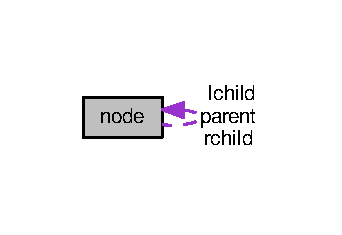
\includegraphics[width=164pt]{structnode__coll__graph}
\end{center}
\end{figure}
\subsection*{Public Types}
\begin{DoxyCompactItemize}
\item 
\hypertarget{structnode_affe9650e53b0efaa6d69372b45d795bd}{enum \{ {\bfseries black}, 
{\bfseries red}
 \}}\label{structnode_affe9650e53b0efaa6d69372b45d795bd}

\end{DoxyCompactItemize}
\subsection*{Public Attributes}
\begin{DoxyCompactItemize}
\item 
\hypertarget{structnode_a883641a3dd856c38125e6a08db4e66af}{enum node\+:: \{ ... \}  {\bfseries colour}}\label{structnode_a883641a3dd856c38125e6a08db4e66af}

\item 
int \hyperlink{structnode_ac8973feda870a119ccdc25910254db0c}{info}
\item 
struct \hyperlink{structnode}{node} $\ast$ \hyperlink{structnode_a5e9a6db5c18bb131ca4b72a1ff575ad8}{lchild}
\item 
struct \hyperlink{structnode}{node} $\ast$ \hyperlink{structnode_aa1ed9628cfc90de6f68ff88ddf9350fa}{rchild}
\item 
struct \hyperlink{structnode}{node} $\ast$ \hyperlink{structnode_a05e4fe9e0177ba2d8dbd2c487cfddd53}{parent}
\end{DoxyCompactItemize}


\subsection{Member Data Documentation}
\hypertarget{structnode_ac8973feda870a119ccdc25910254db0c}{\index{node@{node}!info@{info}}
\index{info@{info}!node@{node}}
\subsubsection[{info}]{\setlength{\rightskip}{0pt plus 5cm}int node\+::info}}\label{structnode_ac8973feda870a119ccdc25910254db0c}
Stores whether the node is red or black \hypertarget{structnode_a5e9a6db5c18bb131ca4b72a1ff575ad8}{\index{node@{node}!lchild@{lchild}}
\index{lchild@{lchild}!node@{node}}
\subsubsection[{lchild}]{\setlength{\rightskip}{0pt plus 5cm}struct {\bf node}$\ast$ node\+::lchild}}\label{structnode_a5e9a6db5c18bb131ca4b72a1ff575ad8}
Stores the value of the node \hypertarget{structnode_a05e4fe9e0177ba2d8dbd2c487cfddd53}{\index{node@{node}!parent@{parent}}
\index{parent@{parent}!node@{node}}
\subsubsection[{parent}]{\setlength{\rightskip}{0pt plus 5cm}struct {\bf node}$\ast$ node\+::parent}}\label{structnode_a05e4fe9e0177ba2d8dbd2c487cfddd53}
Pointer of the right node \hypertarget{structnode_aa1ed9628cfc90de6f68ff88ddf9350fa}{\index{node@{node}!rchild@{rchild}}
\index{rchild@{rchild}!node@{node}}
\subsubsection[{rchild}]{\setlength{\rightskip}{0pt plus 5cm}struct {\bf node}$\ast$ node\+::rchild}}\label{structnode_aa1ed9628cfc90de6f68ff88ddf9350fa}
Pointer of the left node 

The documentation for this struct was generated from the following file\+:\begin{DoxyCompactItemize}
\item 
\hyperlink{red__black__tree_8c}{red\+\_\+black\+\_\+tree.\+c}\end{DoxyCompactItemize}

\hypertarget{structnodef}{}\section{nodef Struct Reference}
\label{structnodef}\index{nodef@{nodef}}


$\ast$-\/-\/-\/-\/-\/-\/-\/-\/-\/-\/-\/-\/-\/-\/-\/-\/-\/-\/-\/-\/-\/-\/-\/-\/-\/-\/------F\+I\+B\+O\+N\+A\+C\+CI H\+E\+A\+P-\/-\/-\/-\/-\/-\/-\/-\/-\/-\/-\/-\/-\/-\/-\/-\/-\/-\/-\/-\/-\/-\/-\/-\/-\/-\/-\/-\/-\/-\/-\/-\/-\/-\/-\/-\/-\/-\/-\/-\/-\/-\/-\/-\/-\/-\/-\/-\/-\/-\/-\/-\/-\/-\/-\/-\/-\/-\/-\/-\/-\/-\/-\/------$\ast$/  


\subsection*{Public Attributes}
\begin{DoxyCompactItemize}
\item 
int {\bfseries n}\hypertarget{structnodef_a445cba4437e11f5bf779a0b9bd1909a1}{}\label{structnodef_a445cba4437e11f5bf779a0b9bd1909a1}

\item 
int \hyperlink{structnodef_a7d8ce9388f378b24275972f1eaa8d8dd}{index}
\item 
int \hyperlink{structnodef_a0a29ea193cba925e68dbcf3ccc673203}{degree}
\item 
\hyperlink{structnodef}{nodef} $\ast$ \hyperlink{structnodef_aea7c4854fecb939b9a236cfa62dc1db3}{parent}
\item 
\hyperlink{structnodef}{nodef} $\ast$ \hyperlink{structnodef_a03c0d01036bbca579381e8f93df0ad87}{child}
\item 
\hyperlink{structnodef}{nodef} $\ast$ \hyperlink{structnodef_ae257022b5d5765c7cad17fe2af4bd89f}{left}
\item 
\hyperlink{structnodef}{nodef} $\ast$ \hyperlink{structnodef_a4242670aeeda1dc26715fb0f1b63661c}{right}
\item 
char \hyperlink{structnodef_a8a6b8531e0ce2c5ef6d6e1afbcad6440}{mark}
\item 
char {\bfseries C}\hypertarget{structnodef_afa451b49b06f8b28c514d1e7bbaac644}{}\label{structnodef_afa451b49b06f8b28c514d1e7bbaac644}

\end{DoxyCompactItemize}


\subsection{Detailed Description}
$\ast$-\/-\/-\/-\/-\/-\/-\/-\/-\/-\/-\/-\/-\/-\/-\/-\/-\/-\/-\/-\/-\/-\/-\/-\/-\/-\/------F\+I\+B\+O\+N\+A\+C\+CI H\+E\+A\+P-\/-\/-\/-\/-\/-\/-\/-\/-\/-\/-\/-\/-\/-\/-\/-\/-\/-\/-\/-\/-\/-\/-\/-\/-\/-\/-\/-\/-\/-\/-\/-\/-\/-\/-\/-\/-\/-\/-\/-\/-\/-\/-\/-\/-\/-\/-\/-\/-\/-\/-\/-\/-\/-\/-\/-\/-\/-\/-\/-\/-\/-\/-\/------$\ast$/ 

Strucure of a node, used to store various info about node in a F\+I\+B\+O\+N\+A\+C\+CI Heap. 

\subsection{Member Data Documentation}
\index{nodef@{nodef}!child@{child}}
\index{child@{child}!nodef@{nodef}}
\subsubsection[{\texorpdfstring{child}{child}}]{\setlength{\rightskip}{0pt plus 5cm}{\bf nodef}$\ast$ nodef\+::child}\hypertarget{structnodef_a03c0d01036bbca579381e8f93df0ad87}{}\label{structnodef_a03c0d01036bbca579381e8f93df0ad87}
Pointer to parent of the node \index{nodef@{nodef}!degree@{degree}}
\index{degree@{degree}!nodef@{nodef}}
\subsubsection[{\texorpdfstring{degree}{degree}}]{\setlength{\rightskip}{0pt plus 5cm}int nodef\+::degree}\hypertarget{structnodef_a0a29ea193cba925e68dbcf3ccc673203}{}\label{structnodef_a0a29ea193cba925e68dbcf3ccc673203}
Index of the node \index{nodef@{nodef}!index@{index}}
\index{index@{index}!nodef@{nodef}}
\subsubsection[{\texorpdfstring{index}{index}}]{\setlength{\rightskip}{0pt plus 5cm}int nodef\+::index}\hypertarget{structnodef_a7d8ce9388f378b24275972f1eaa8d8dd}{}\label{structnodef_a7d8ce9388f378b24275972f1eaa8d8dd}
Stores value of the node \index{nodef@{nodef}!left@{left}}
\index{left@{left}!nodef@{nodef}}
\subsubsection[{\texorpdfstring{left}{left}}]{\setlength{\rightskip}{0pt plus 5cm}{\bf nodef}$\ast$ nodef\+::left}\hypertarget{structnodef_ae257022b5d5765c7cad17fe2af4bd89f}{}\label{structnodef_ae257022b5d5765c7cad17fe2af4bd89f}
Pointer to child of the node \index{nodef@{nodef}!mark@{mark}}
\index{mark@{mark}!nodef@{nodef}}
\subsubsection[{\texorpdfstring{mark}{mark}}]{\setlength{\rightskip}{0pt plus 5cm}char nodef\+::mark}\hypertarget{structnodef_a8a6b8531e0ce2c5ef6d6e1afbcad6440}{}\label{structnodef_a8a6b8531e0ce2c5ef6d6e1afbcad6440}
Pointer to right child of the node \index{nodef@{nodef}!parent@{parent}}
\index{parent@{parent}!nodef@{nodef}}
\subsubsection[{\texorpdfstring{parent}{parent}}]{\setlength{\rightskip}{0pt plus 5cm}{\bf nodef}$\ast$ nodef\+::parent}\hypertarget{structnodef_aea7c4854fecb939b9a236cfa62dc1db3}{}\label{structnodef_aea7c4854fecb939b9a236cfa62dc1db3}
Degree of the node \index{nodef@{nodef}!right@{right}}
\index{right@{right}!nodef@{nodef}}
\subsubsection[{\texorpdfstring{right}{right}}]{\setlength{\rightskip}{0pt plus 5cm}{\bf nodef}$\ast$ nodef\+::right}\hypertarget{structnodef_a4242670aeeda1dc26715fb0f1b63661c}{}\label{structnodef_a4242670aeeda1dc26715fb0f1b63661c}
Pointer to left child of the node 

The documentation for this struct was generated from the following file\+:\begin{DoxyCompactItemize}
\item 
\hyperlink{dijkstra_8cpp}{dijkstra.\+cpp}\end{DoxyCompactItemize}

\chapter{File Documentation}
\hypertarget{dijkstra_8cpp}{}\section{dijkstra.\+cpp File Reference}
\label{dijkstra_8cpp}\index{dijkstra.\+cpp@{dijkstra.\+cpp}}


Implementation of Dijsktra\textquotesingle{}s algorithm using Binary Heap, Binomial Heap and Fibonacci Heap.  


{\ttfamily \#include $<$bits/stdc++.\+h$>$}\\*
\subsection*{Classes}
\begin{DoxyCompactItemize}
\item 
struct \hyperlink{structnode}{node}
\begin{DoxyCompactList}\small\item\em $\ast$-\/-\/-\/-\/-\/-\/-\/-\/-\/-\/-\/-\/-\/-\/-\/-\/-\/-\/-\/-\/-\/-\/-\/-\/-\/------B\+I\+N\+O\+M\+I\+AL H\+E\+A\+P-\/-\/-\/-\/-\/-\/-\/-\/-\/-\/-\/-\/-\/-\/-\/-\/-\/-\/-\/-\/-\/-\/-\/-\/-\/-\/-\/-\/-\/-\/-\/-\/-\/-\/-\/-\/-\/-\/-\/-\/-\/-\/-\/-\/-\/-\/-\/-\/-\/-\/------$\ast$/ \end{DoxyCompactList}\item 
class \hyperlink{classBinomialHeap}{Binomial\+Heap}
\begin{DoxyCompactList}\small\item\em Binomial Heap Data Structure class. \end{DoxyCompactList}\item 
struct \hyperlink{structnodef}{nodef}
\begin{DoxyCompactList}\small\item\em $\ast$-\/-\/-\/-\/-\/-\/-\/-\/-\/-\/-\/-\/-\/-\/-\/-\/-\/-\/-\/-\/-\/-\/-\/-\/-\/-\/------F\+I\+B\+O\+N\+A\+C\+CI H\+E\+A\+P-\/-\/-\/-\/-\/-\/-\/-\/-\/-\/-\/-\/-\/-\/-\/-\/-\/-\/-\/-\/-\/-\/-\/-\/-\/-\/-\/-\/-\/-\/-\/-\/-\/-\/-\/-\/-\/-\/-\/-\/-\/-\/-\/-\/-\/-\/-\/-\/-\/-\/-\/-\/-\/-\/-\/-\/-\/-\/-\/-\/-\/-\/-\/------$\ast$/ \end{DoxyCompactList}\item 
class \hyperlink{classFibonacciHeap}{Fibonacci\+Heap}
\begin{DoxyCompactList}\small\item\em Fibonacci Heap Data Structure class. \end{DoxyCompactList}\end{DoxyCompactItemize}
\subsection*{Macros}
\begin{DoxyCompactItemize}
\item 
\#define {\bfseries M\+AX}~100001\hypertarget{dijkstra_8cpp_a392fb874e547e582e9c66a08a1f23326}{}\label{dijkstra_8cpp_a392fb874e547e582e9c66a08a1f23326}

\item 
\#define {\bfseries I\+NF}~(1$<$$<$20)\hypertarget{dijkstra_8cpp_a12c2040f25d8e3a7b9e1c2024c618cb6}{}\label{dijkstra_8cpp_a12c2040f25d8e3a7b9e1c2024c618cb6}

\item 
\#define {\bfseries pii}~pair$<$ int, int $>$\hypertarget{dijkstra_8cpp_ad665d3545da459160ac2b774063cc367}{}\label{dijkstra_8cpp_ad665d3545da459160ac2b774063cc367}

\item 
\#define {\bfseries pb}(x)~push\+\_\+back(x)\hypertarget{dijkstra_8cpp_a718dd9f88a8a951fe6b91f9fffaee305}{}\label{dijkstra_8cpp_a718dd9f88a8a951fe6b91f9fffaee305}

\end{DoxyCompactItemize}
\subsection*{Functions}
\begin{DoxyCompactItemize}
\item 
int \hyperlink{dijkstra_8cpp_ab0f4486e55f1ff205438507d914d87e1}{parent} (int index)
\begin{DoxyCompactList}\small\item\em Finds the parent of a node in a tree. \end{DoxyCompactList}\item 
int \hyperlink{dijkstra_8cpp_a433986963774dd5b1a942a7fa6b9a07f}{value} (int index)
\begin{DoxyCompactList}\small\item\em Returns the value of the node for a fiven index. \end{DoxyCompactList}\item 
void \hyperlink{dijkstra_8cpp_af96b1b6618a0c4cfd630ea59e8506bd0}{heapify\+Up\+Binary\+Heap} (int index)
\begin{DoxyCompactList}\small\item\em Heapifies the given binary heap after insertion or deletion. Min Heap. \end{DoxyCompactList}\item 
void \hyperlink{dijkstra_8cpp_a9ab56ec361175aa7ab085057afb804bc}{insert\+Binary\+Heap} (pair$<$ int, int $>$ element)
\begin{DoxyCompactList}\small\item\em Insertion of a new node in the given Binary Heap. \end{DoxyCompactList}\item 
int \hyperlink{dijkstra_8cpp_aa27ffacff065847b3421ace4958ea782}{get\+Left} (int index)
\begin{DoxyCompactList}\small\item\em Gets the left child index of a given node. \end{DoxyCompactList}\item 
int \hyperlink{dijkstra_8cpp_a55aa54819a680f161719d3c18028a7f8}{get\+Right} (int index)
\begin{DoxyCompactList}\small\item\em Gets the right child index of a given node. \end{DoxyCompactList}\item 
void \hyperlink{dijkstra_8cpp_a9e95a41df12e4ca165a350fca66659e4}{heapify\+Down\+Binary\+Heap} (int index)
\begin{DoxyCompactList}\small\item\em Heapify the binary heap after Deleion Operation (Sort) \end{DoxyCompactList}\item 
pair$<$ int, int $>$ \hyperlink{dijkstra_8cpp_af2de7bf96c6575abe364eec181958d1f}{delete\+Binary\+Heap} ()
\begin{DoxyCompactList}\small\item\em Obtains the lowest value from the heap and deleted the node and then heapifies the binary heap. \end{DoxyCompactList}\item 
void \hyperlink{dijkstra_8cpp_a5385191f1fa49e3bff8f8454ec06d4b7}{binary\+\_\+heap} ()
\begin{DoxyCompactList}\small\item\em Create a Binary Heap. \end{DoxyCompactList}\item 
void \hyperlink{dijkstra_8cpp_a65b63d3256f123d625130e6a4bb2181f}{binomial\+\_\+heap} ()
\begin{DoxyCompactList}\small\item\em Create a Binomial Heap. \end{DoxyCompactList}\item 
void \hyperlink{dijkstra_8cpp_a5a1be60286c4d631fcdc294d63406f90}{fibonacci\+\_\+heap} ()
\begin{DoxyCompactList}\small\item\em Create a F\+I\+B\+O\+N\+A\+C\+CI Heap. \end{DoxyCompactList}\item 
int \hyperlink{dijkstra_8cpp_ae66f6b31b5ad750f1fe042a706a4e3d4}{main} ()
\begin{DoxyCompactList}\small\item\em The Main Function of the Program. \end{DoxyCompactList}\end{DoxyCompactItemize}
\subsection*{Variables}
\begin{DoxyCompactItemize}
\item 
int {\bfseries index\+\_\+node}\hypertarget{dijkstra_8cpp_a083793c1b5128f65f2800cc8dc7087bb}{}\label{dijkstra_8cpp_a083793c1b5128f65f2800cc8dc7087bb}

\item 
vector$<$ pair$<$ int, int $>$ $>$ \hyperlink{dijkstra_8cpp_a8ba291d491dc90547eae0d456cb3c44c}{binary\+Heap}\hypertarget{dijkstra_8cpp_a8ba291d491dc90547eae0d456cb3c44c}{}\label{dijkstra_8cpp_a8ba291d491dc90547eae0d456cb3c44c}

\begin{DoxyCompactList}\small\item\em $\ast$-\/-\/-\/-\/-\/-\/-\/-\/-\/-\/-\/-\/-\/-\/-\/-\/-\/-\/-\/-\/-\/-\/-\/-\/-\/-\/-\/-\/---B\+I\+N\+A\+RY H\+E\+A\+P-\/-\/-\/-\/-\/-\/-\/-\/-\/-\/-\/-\/-\/-\/-\/-\/-\/-\/-\/-\/-\/-\/-\/-\/-\/-\/-\/-\/-\/-\/-\/-\/-\/-\/-\/-\/-\/-\/-\/-\/-\/-\/-\/-\/-\/-\/-\/-\/-\/-\/-\/-\/-\/-\/-\/---$\ast$/ \end{DoxyCompactList}\item 
vector$<$ pii $>$ {\bfseries G} \mbox{[}M\+AX\mbox{]}\hypertarget{dijkstra_8cpp_a29a3f1b4fd7c22f5a897888b932f98ab}{}\label{dijkstra_8cpp_a29a3f1b4fd7c22f5a897888b932f98ab}

\item 
int {\bfseries D} \mbox{[}M\+AX\mbox{]}\hypertarget{dijkstra_8cpp_a41eed31ede9e206d8f69a3601a2875bd}{}\label{dijkstra_8cpp_a41eed31ede9e206d8f69a3601a2875bd}

\item 
bool {\bfseries F} \mbox{[}M\+AX\mbox{]}\hypertarget{dijkstra_8cpp_a13f197341dfce548b9f9584d441b828d}{}\label{dijkstra_8cpp_a13f197341dfce548b9f9584d441b828d}

\item 
int {\bfseries i}\hypertarget{dijkstra_8cpp_acb559820d9ca11295b4500f179ef6392}{}\label{dijkstra_8cpp_acb559820d9ca11295b4500f179ef6392}

\item 
int {\bfseries u}\hypertarget{dijkstra_8cpp_a5874b4c2ec2e28321eea4e4871d08222}{}\label{dijkstra_8cpp_a5874b4c2ec2e28321eea4e4871d08222}

\item 
int {\bfseries v}\hypertarget{dijkstra_8cpp_ac8859e8c1ce357c4c8b37bbb1936ba1c}{}\label{dijkstra_8cpp_ac8859e8c1ce357c4c8b37bbb1936ba1c}

\item 
int {\bfseries w}\hypertarget{dijkstra_8cpp_aac374e320caaadeca4874add33b62af2}{}\label{dijkstra_8cpp_aac374e320caaadeca4874add33b62af2}

\item 
int {\bfseries sz}\hypertarget{dijkstra_8cpp_a0e1ea19fb9fa7881d15d84eff4c090e1}{}\label{dijkstra_8cpp_a0e1ea19fb9fa7881d15d84eff4c090e1}

\item 
int {\bfseries nodes}\hypertarget{dijkstra_8cpp_a6b7983ccd32c86cbbc3d4d9cda4cac17}{}\label{dijkstra_8cpp_a6b7983ccd32c86cbbc3d4d9cda4cac17}

\item 
int {\bfseries edges}\hypertarget{dijkstra_8cpp_a398acefd9cbf90d7f477b65d55a6b1ec}{}\label{dijkstra_8cpp_a398acefd9cbf90d7f477b65d55a6b1ec}

\item 
int {\bfseries starting}\hypertarget{dijkstra_8cpp_ae3e9c2dd4477c3dbccc953a5dc27da6f}{}\label{dijkstra_8cpp_ae3e9c2dd4477c3dbccc953a5dc27da6f}

\end{DoxyCompactItemize}


\subsection{Detailed Description}
Implementation of Dijsktra\textquotesingle{}s algorithm using Binary Heap, Binomial Heap and Fibonacci Heap. 

\begin{DoxyDate}{Date}
15 April 2016
\end{DoxyDate}
\begin{DoxyAuthor}{Author}
Shrukul Habib 13\+C\+O143 

Anant Maheshwari 13\+C\+O111 
\end{DoxyAuthor}


\subsection{Function Documentation}
\index{dijkstra.\+cpp@{dijkstra.\+cpp}!binary\+\_\+heap@{binary\+\_\+heap}}
\index{binary\+\_\+heap@{binary\+\_\+heap}!dijkstra.\+cpp@{dijkstra.\+cpp}}
\subsubsection[{\texorpdfstring{binary\+\_\+heap()}{binary_heap()}}]{\setlength{\rightskip}{0pt plus 5cm}void binary\+\_\+heap (
\begin{DoxyParamCaption}
{}
\end{DoxyParamCaption}
)}\hypertarget{dijkstra_8cpp_a5385191f1fa49e3bff8f8454ec06d4b7}{}\label{dijkstra_8cpp_a5385191f1fa49e3bff8f8454ec06d4b7}


Create a Binary Heap. 

\begin{DoxyReturn}{Returns}
Returns void 
\end{DoxyReturn}
\index{dijkstra.\+cpp@{dijkstra.\+cpp}!binomial\+\_\+heap@{binomial\+\_\+heap}}
\index{binomial\+\_\+heap@{binomial\+\_\+heap}!dijkstra.\+cpp@{dijkstra.\+cpp}}
\subsubsection[{\texorpdfstring{binomial\+\_\+heap()}{binomial_heap()}}]{\setlength{\rightskip}{0pt plus 5cm}void binomial\+\_\+heap (
\begin{DoxyParamCaption}
{}
\end{DoxyParamCaption}
)}\hypertarget{dijkstra_8cpp_a65b63d3256f123d625130e6a4bb2181f}{}\label{dijkstra_8cpp_a65b63d3256f123d625130e6a4bb2181f}


Create a Binomial Heap. 

\begin{DoxyReturn}{Returns}
Returns void 
\end{DoxyReturn}
\index{dijkstra.\+cpp@{dijkstra.\+cpp}!delete\+Binary\+Heap@{delete\+Binary\+Heap}}
\index{delete\+Binary\+Heap@{delete\+Binary\+Heap}!dijkstra.\+cpp@{dijkstra.\+cpp}}
\subsubsection[{\texorpdfstring{delete\+Binary\+Heap()}{deleteBinaryHeap()}}]{\setlength{\rightskip}{0pt plus 5cm}pair$<$int,int$>$ delete\+Binary\+Heap (
\begin{DoxyParamCaption}
{}
\end{DoxyParamCaption}
)}\hypertarget{dijkstra_8cpp_af2de7bf96c6575abe364eec181958d1f}{}\label{dijkstra_8cpp_af2de7bf96c6575abe364eec181958d1f}


Obtains the lowest value from the heap and deleted the node and then heapifies the binary heap. 

\begin{DoxyReturn}{Returns}
Returns the deleted (minimum-\/valued) node 
\end{DoxyReturn}
\index{dijkstra.\+cpp@{dijkstra.\+cpp}!fibonacci\+\_\+heap@{fibonacci\+\_\+heap}}
\index{fibonacci\+\_\+heap@{fibonacci\+\_\+heap}!dijkstra.\+cpp@{dijkstra.\+cpp}}
\subsubsection[{\texorpdfstring{fibonacci\+\_\+heap()}{fibonacci_heap()}}]{\setlength{\rightskip}{0pt plus 5cm}void fibonacci\+\_\+heap (
\begin{DoxyParamCaption}
{}
\end{DoxyParamCaption}
)}\hypertarget{dijkstra_8cpp_a5a1be60286c4d631fcdc294d63406f90}{}\label{dijkstra_8cpp_a5a1be60286c4d631fcdc294d63406f90}


Create a F\+I\+B\+O\+N\+A\+C\+CI Heap. 

\begin{DoxyReturn}{Returns}
Returns void 
\end{DoxyReturn}
\index{dijkstra.\+cpp@{dijkstra.\+cpp}!get\+Left@{get\+Left}}
\index{get\+Left@{get\+Left}!dijkstra.\+cpp@{dijkstra.\+cpp}}
\subsubsection[{\texorpdfstring{get\+Left(int index)}{getLeft(int index)}}]{\setlength{\rightskip}{0pt plus 5cm}int get\+Left (
\begin{DoxyParamCaption}
\item[{int}]{index}
\end{DoxyParamCaption}
)}\hypertarget{dijkstra_8cpp_aa27ffacff065847b3421ace4958ea782}{}\label{dijkstra_8cpp_aa27ffacff065847b3421ace4958ea782}


Gets the left child index of a given node. 


\begin{DoxyParams}{Parameters}
{\em index} & The index of the node whose left child is to be found \\
\hline
\end{DoxyParams}
\begin{DoxyReturn}{Returns}
Returns the index of the left child of the given node 
\end{DoxyReturn}
\index{dijkstra.\+cpp@{dijkstra.\+cpp}!get\+Right@{get\+Right}}
\index{get\+Right@{get\+Right}!dijkstra.\+cpp@{dijkstra.\+cpp}}
\subsubsection[{\texorpdfstring{get\+Right(int index)}{getRight(int index)}}]{\setlength{\rightskip}{0pt plus 5cm}int get\+Right (
\begin{DoxyParamCaption}
\item[{int}]{index}
\end{DoxyParamCaption}
)}\hypertarget{dijkstra_8cpp_a55aa54819a680f161719d3c18028a7f8}{}\label{dijkstra_8cpp_a55aa54819a680f161719d3c18028a7f8}


Gets the right child index of a given node. 


\begin{DoxyParams}{Parameters}
{\em index} & The index of the node whose right child is to be found \\
\hline
\end{DoxyParams}
\begin{DoxyReturn}{Returns}
Returns the index of the right child of the given node 
\end{DoxyReturn}
\index{dijkstra.\+cpp@{dijkstra.\+cpp}!heapify\+Down\+Binary\+Heap@{heapify\+Down\+Binary\+Heap}}
\index{heapify\+Down\+Binary\+Heap@{heapify\+Down\+Binary\+Heap}!dijkstra.\+cpp@{dijkstra.\+cpp}}
\subsubsection[{\texorpdfstring{heapify\+Down\+Binary\+Heap(int index)}{heapifyDownBinaryHeap(int index)}}]{\setlength{\rightskip}{0pt plus 5cm}void heapify\+Down\+Binary\+Heap (
\begin{DoxyParamCaption}
\item[{int}]{index}
\end{DoxyParamCaption}
)}\hypertarget{dijkstra_8cpp_a9e95a41df12e4ca165a350fca66659e4}{}\label{dijkstra_8cpp_a9e95a41df12e4ca165a350fca66659e4}


Heapify the binary heap after Deleion Operation (Sort) 


\begin{DoxyParams}{Parameters}
{\em index} & The index of the node from which the the heapify operation begins, called the function with parameter 0 initially \\
\hline
\end{DoxyParams}
\begin{DoxyReturn}{Returns}
Doesn\textquotesingle{}t return anything, void 
\end{DoxyReturn}
\index{dijkstra.\+cpp@{dijkstra.\+cpp}!heapify\+Up\+Binary\+Heap@{heapify\+Up\+Binary\+Heap}}
\index{heapify\+Up\+Binary\+Heap@{heapify\+Up\+Binary\+Heap}!dijkstra.\+cpp@{dijkstra.\+cpp}}
\subsubsection[{\texorpdfstring{heapify\+Up\+Binary\+Heap(int index)}{heapifyUpBinaryHeap(int index)}}]{\setlength{\rightskip}{0pt plus 5cm}void heapify\+Up\+Binary\+Heap (
\begin{DoxyParamCaption}
\item[{int}]{index}
\end{DoxyParamCaption}
)}\hypertarget{dijkstra_8cpp_af96b1b6618a0c4cfd630ea59e8506bd0}{}\label{dijkstra_8cpp_af96b1b6618a0c4cfd630ea59e8506bd0}


Heapifies the given binary heap after insertion or deletion. Min Heap. 


\begin{DoxyParams}{Parameters}
{\em index} & The index of the node where any operation was made \\
\hline
\end{DoxyParams}
\begin{DoxyReturn}{Returns}
Doesn\textquotesingle{}t return anything, void 
\end{DoxyReturn}
\index{dijkstra.\+cpp@{dijkstra.\+cpp}!insert\+Binary\+Heap@{insert\+Binary\+Heap}}
\index{insert\+Binary\+Heap@{insert\+Binary\+Heap}!dijkstra.\+cpp@{dijkstra.\+cpp}}
\subsubsection[{\texorpdfstring{insert\+Binary\+Heap(pair$<$ int, int $>$ element)}{insertBinaryHeap(pair< int, int > element)}}]{\setlength{\rightskip}{0pt plus 5cm}void insert\+Binary\+Heap (
\begin{DoxyParamCaption}
\item[{pair$<$ int, int $>$}]{element}
\end{DoxyParamCaption}
)}\hypertarget{dijkstra_8cpp_a9ab56ec361175aa7ab085057afb804bc}{}\label{dijkstra_8cpp_a9ab56ec361175aa7ab085057afb804bc}


Insertion of a new node in the given Binary Heap. 


\begin{DoxyParams}{Parameters}
{\em element} & the value and the index of the new node to be inserted combined in pair data structure \\
\hline
\end{DoxyParams}
\begin{DoxyReturn}{Returns}
Doesn\textquotesingle{}t return anything, void 
\end{DoxyReturn}
\index{dijkstra.\+cpp@{dijkstra.\+cpp}!main@{main}}
\index{main@{main}!dijkstra.\+cpp@{dijkstra.\+cpp}}
\subsubsection[{\texorpdfstring{main()}{main()}}]{\setlength{\rightskip}{0pt plus 5cm}int main (
\begin{DoxyParamCaption}
{}
\end{DoxyParamCaption}
)}\hypertarget{dijkstra_8cpp_ae66f6b31b5ad750f1fe042a706a4e3d4}{}\label{dijkstra_8cpp_ae66f6b31b5ad750f1fe042a706a4e3d4}


The Main Function of the Program. 

\begin{DoxyReturn}{Returns}
Return int value 
\end{DoxyReturn}
\index{dijkstra.\+cpp@{dijkstra.\+cpp}!parent@{parent}}
\index{parent@{parent}!dijkstra.\+cpp@{dijkstra.\+cpp}}
\subsubsection[{\texorpdfstring{parent(int index)}{parent(int index)}}]{\setlength{\rightskip}{0pt plus 5cm}int parent (
\begin{DoxyParamCaption}
\item[{int}]{index}
\end{DoxyParamCaption}
)}\hypertarget{dijkstra_8cpp_ab0f4486e55f1ff205438507d914d87e1}{}\label{dijkstra_8cpp_ab0f4486e55f1ff205438507d914d87e1}


Finds the parent of a node in a tree. 


\begin{DoxyParams}{Parameters}
{\em index} & The index of the node whose parent is to be found \\
\hline
\end{DoxyParams}
\begin{DoxyReturn}{Returns}
returns the index of the parent if it exist, if the node is the root, then returns -\/1 
\end{DoxyReturn}
\index{dijkstra.\+cpp@{dijkstra.\+cpp}!value@{value}}
\index{value@{value}!dijkstra.\+cpp@{dijkstra.\+cpp}}
\subsubsection[{\texorpdfstring{value(int index)}{value(int index)}}]{\setlength{\rightskip}{0pt plus 5cm}int value (
\begin{DoxyParamCaption}
\item[{int}]{index}
\end{DoxyParamCaption}
)}\hypertarget{dijkstra_8cpp_a433986963774dd5b1a942a7fa6b9a07f}{}\label{dijkstra_8cpp_a433986963774dd5b1a942a7fa6b9a07f}


Returns the value of the node for a fiven index. 


\begin{DoxyParams}{Parameters}
{\em index} & The index of the node whose value is to be found \\
\hline
\end{DoxyParams}
\begin{DoxyReturn}{Returns}
returns the value of the node for the given index 
\end{DoxyReturn}

%--- End generated contents ---

% Index
\backmatter
\newpage
\phantomsection
\clearemptydoublepage
\addcontentsline{toc}{chapter}{Index}
\printindex

\end{document}
